\hypertarget{introduction}{%
\subsection{Introduction}\label{introduction}}

\#TODO

\begin{center}\rule{0.5\linewidth}{0.5pt}\end{center}

\textbf{1 -- Generative Adversarial Networks} \#\# 1. Interpret the
equations (6) and (7). What would happen if we only used one of the two?
If we use only the loss of the equation (6) than the discriminator will
not improve, therefore the generator will easily fool the discriminator
and generate bad looking images. If we only use equation (7) than the
generator will not improve, therefore it will not pass the discriminator
check. \#\# 2. Ideally, what should the generator G transform the
distribution P (z) to? Ideally the the generator should sample new
images that can fool the discriminator check and that are similar to the
ones in the train set but also original. \#\# 3. Remark that the
equation (6) is not directly derived from the equation 5. This is
justified by the authors to obtain more stable training and avoid the
saturation of gradients. What should the ``true'' equation be here ?
Normally the loss function is this:
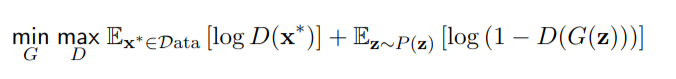
\includegraphics{./images/Pasted image 20231213162826.png} so for the G
the important part would be: \[ min_G = E_{z\sim P(z)}log(1-D(G(z)))\]
The equation used by the authors is used in order to avoid the vanishing
gradient problem: during the optimization process if we calculate the
gradient of this part of the loss it would look like this:
\[D[log(1-D(G(z)))] = D[\frac{1}{(1-\sigma)}\sigma] = \frac{\sigma(1-\sigma)}{(1-\sigma)} = \sigma\]
And at the beginning this would be closer to zero.

Instead if we rewrite this loss as: \[max_G = log(D(G(z)))\] then the
derivation would be:
\[D[log(D(G(z)))] = \frac{1}{(\sigma)}\sigma(1-\sigma) = 1 -\sigma\]
which in the beginning would be going to 1

\hypertarget{comment-on-the-training-of-of-the-gan-with-the-default-settings-progress-of-the-generations-the-loss-stability-image-diversity-etc.}{%
\subsection{4. Comment on the training of of the GAN with the default
settings (progress of the generations, the loss, stability, image
diversity,
etc.}\label{comment-on-the-training-of-of-the-gan-with-the-default-settings-progress-of-the-generations-the-loss-stability-image-diversity-etc.}}

We train our network with the given parameters, and we obtain images
that are quite good and diverse. The loss curves of the generator and
discriminator are not stable because the two networks are adversaries.
When the generator's loss decreases, the discriminator's loss increases,
and vice versa. This is because they are in a continual adversarial
competition -- when one network tries to reduce its loss, the other
network responds by attempting to increase it, creating a dynamic and
fluctuating relationship.

\emph{\textbf{Baseline}:} \emph{ngf=32 -\textgreater{} Channel size
before the last layer in Generator} \emph{ndf=32 -\textgreater{} Channel
size in Discriminator} \emph{weight\_init=``custom'' -\textgreater{}
Weight initialization type} \emph{loss\_type=default -\textgreater{}
Type of training loss for the generator} \emph{lr\_d=0.0002
-\textgreater{} Learning rate for the discriminator} \emph{lr\_g=0.0005
-\textgreater{} Learning rate for the generator} \emph{beta1=0.5
-\textgreater{} Beta1 for Adam optimizer} \emph{epochs=5 -\textgreater{}
Number of training epochs} \emph{nz=100 -\textgreater{} Latent size}
\emph{batch\_size=12 -\textgreater{} Batch size} \emph{nchannels=1
-\textgreater{} Number of channels for inputs of Discriminator}

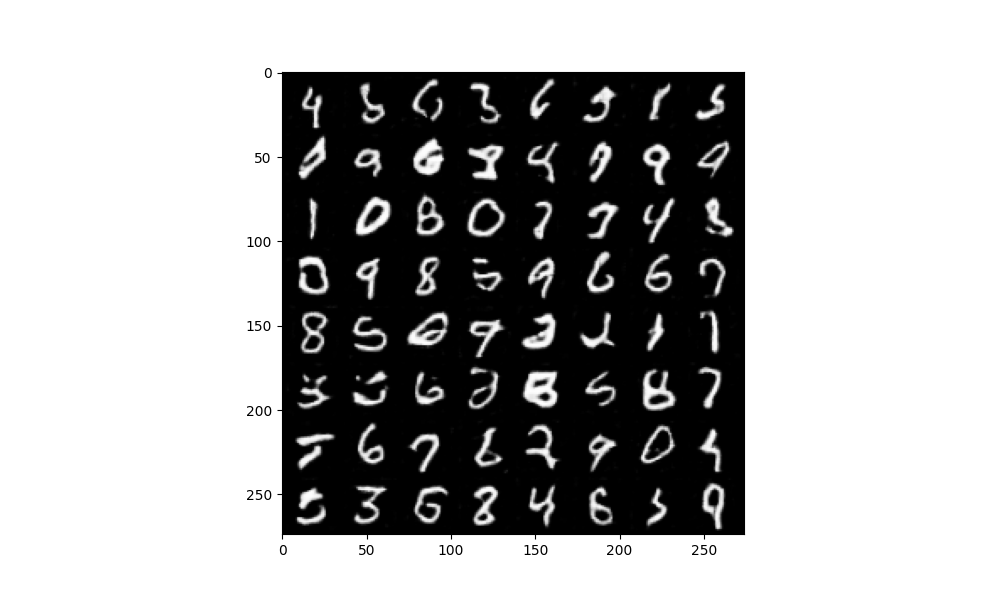
\includegraphics{./images/Pasted image 20231228111114.png}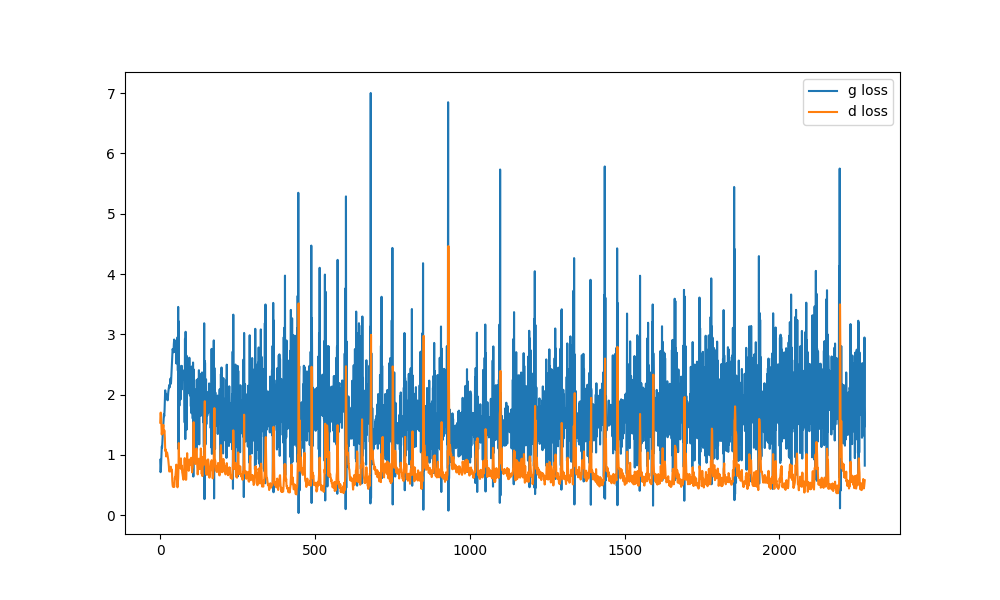
\includegraphics{./images/Pasted image 20231228112219.png}

\hypertarget{comment-on-the-diverse-experiences-that-you-have-performed-with-the-suggestions-above.-in-particular-comment-on-the-stability-on-training-the-losses-the-diversity-of-generated-images-etc.}{%
\subsection{5. Comment on the diverse experiences that you have
performed with the suggestions above. In particular, comment on the
stability on training, the losses, the diversity of generated images,
etc.}\label{comment-on-the-diverse-experiences-that-you-have-performed-with-the-suggestions-above.-in-particular-comment-on-the-stability-on-training-the-losses-the-diversity-of-generated-images-etc.}}

\textbf{Modify ngf or ndf. In particular, reduce or increase one of the
two significantly.} Starting with ngf, if we increase it, we will not
obtain significant differences between the baseline. We can see that the
discriminator perform a little bit worse that the generator when
increasing ndf and also the training seems more stable. ngf=64
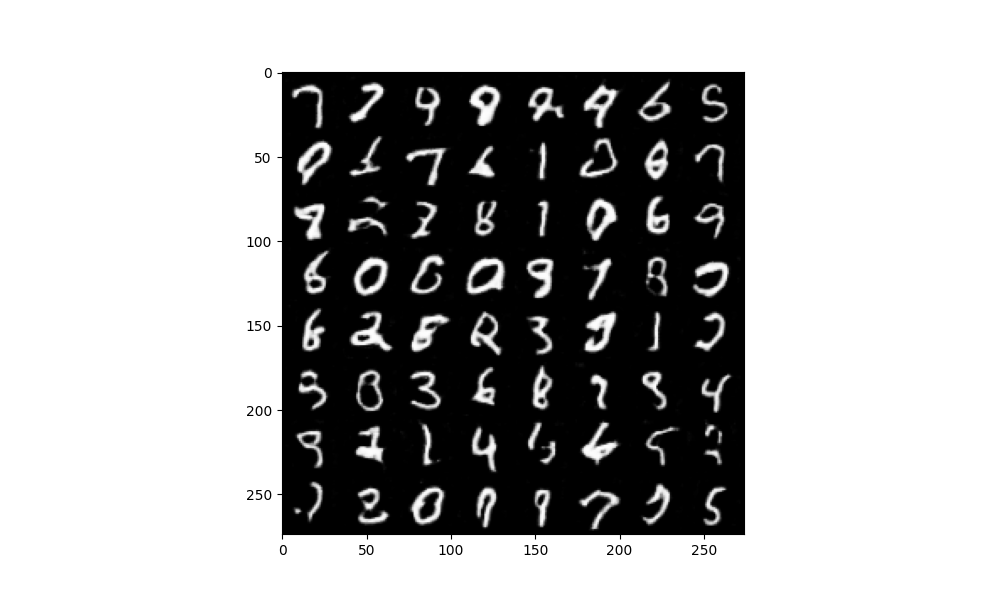
\includegraphics{./images/Pasted image 20231228113811.png}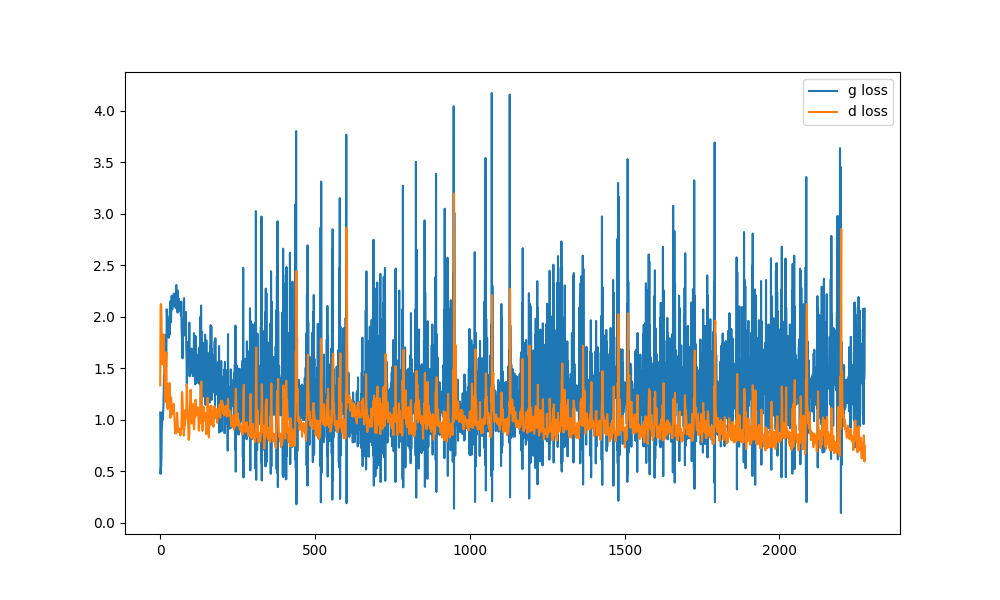
\includegraphics{./images/Pasted image 20231228113841.png}
ngf=128
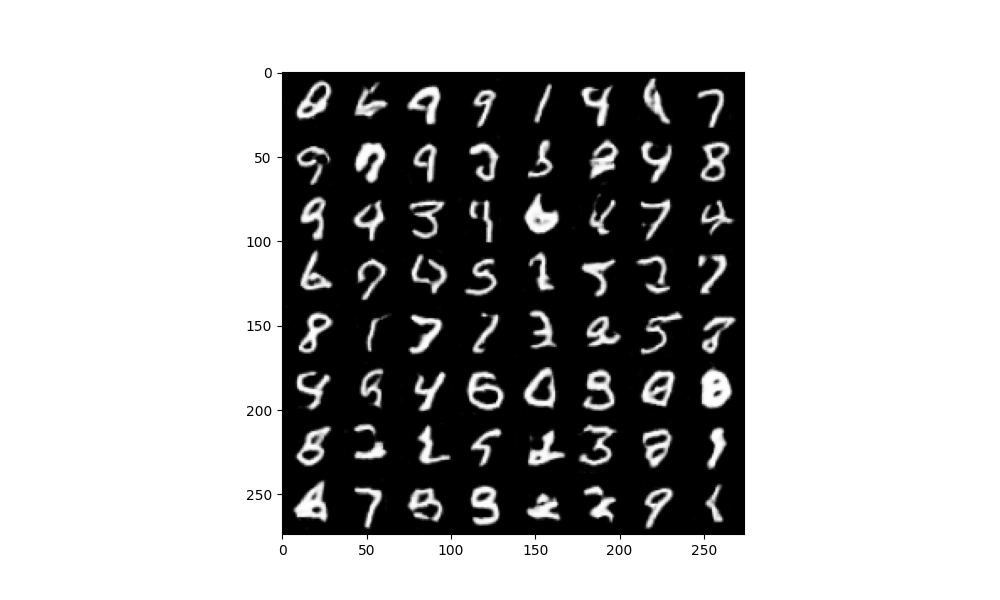
\includegraphics{./images/Pasted image 20231228113921.png}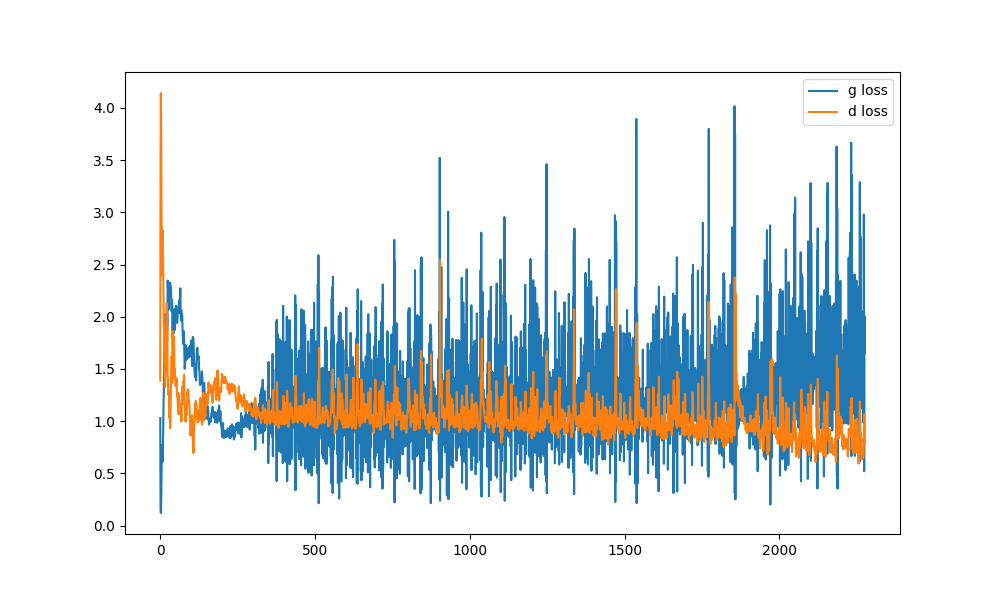
\includegraphics{./images/Pasted image 20231228113936.png}
ngf=256
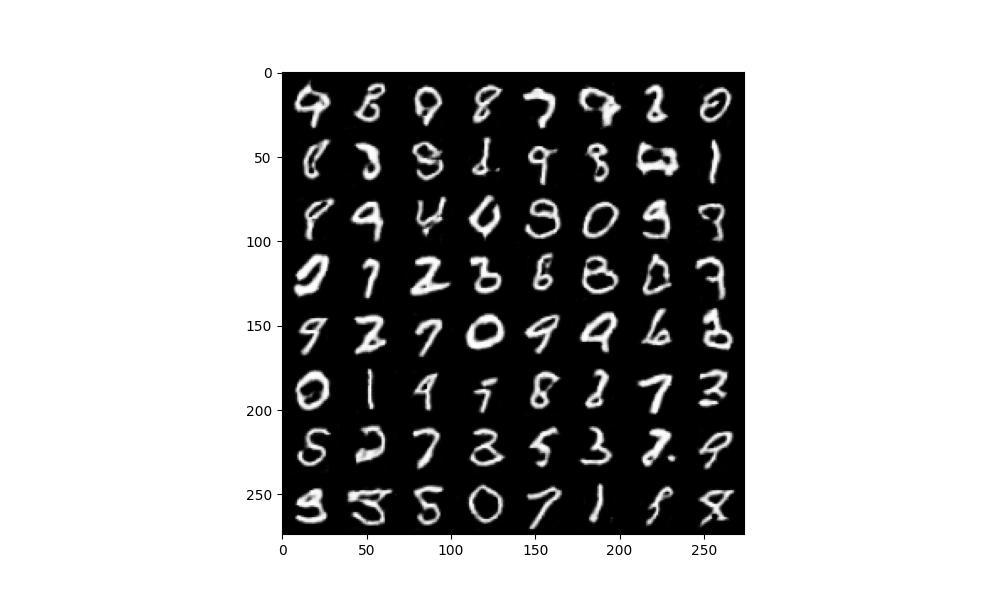
\includegraphics{./images/Pasted image 20231228114012.png}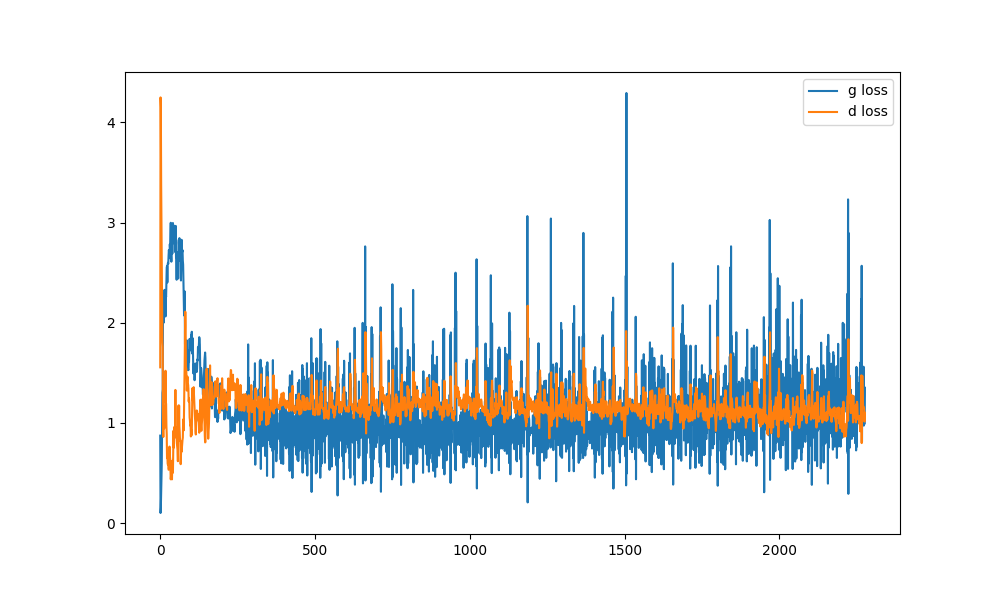
\includegraphics{./images/Pasted image 20231228114031.png}

While, increasing the ndf will produce different results: at ndf=256 the
performances drop significantly. We can see that the generator loss
perform poorer and poorer each time we increase ndf. One explanation
could be that the discriminator becomes too powerful compared to the
generator (i.e., it has a higher capacity). Moreover if the
discriminator is too complex, the gradients during backpropagation may
become very small (vanish), making it challenging for the generator to
learn and update its parameters effectively. ndf=64
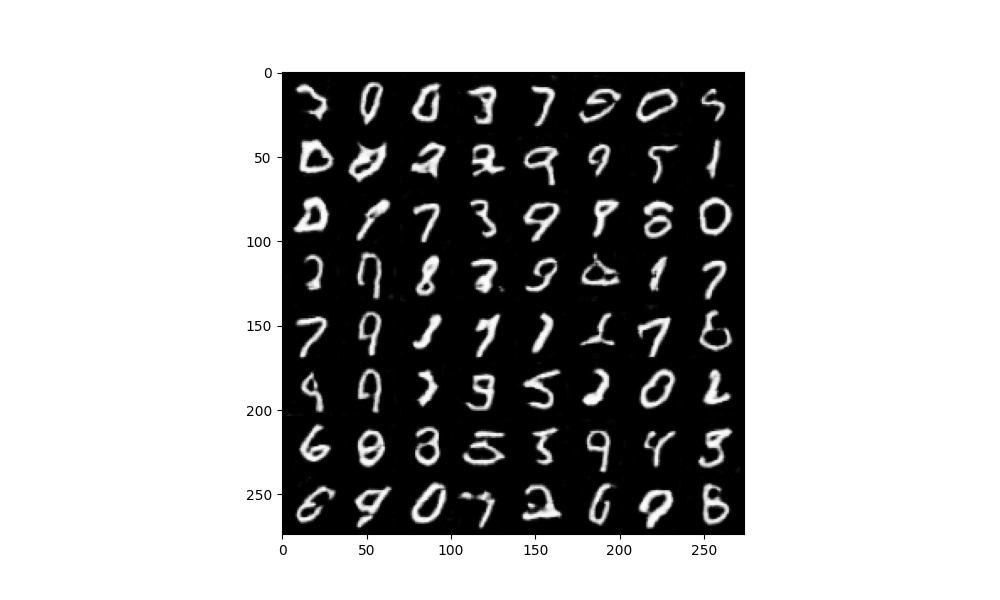
\includegraphics{./images/Pasted image 20231228114134.png}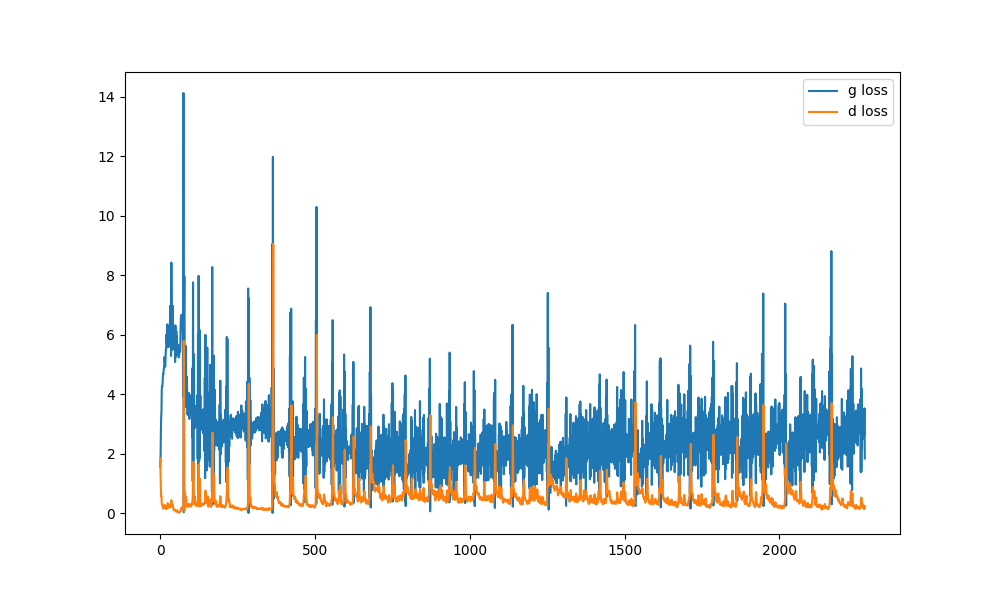
\includegraphics{./images/Pasted image 20231228114145.png}
ndf=128
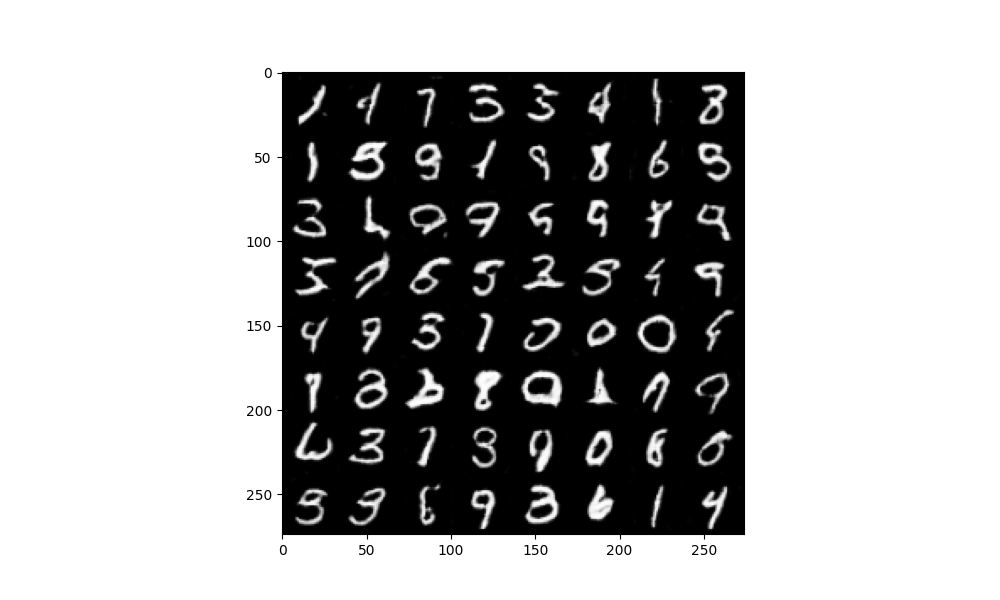
\includegraphics{./images/Pasted image 20231228114224.png}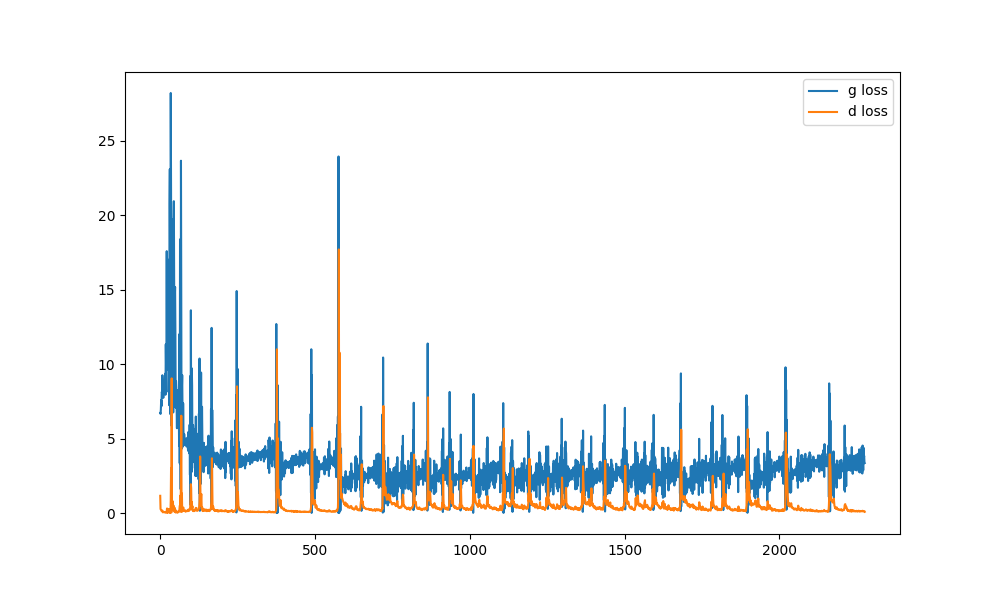
\includegraphics{./images/Pasted image 20231228114234.png}
ndf=256
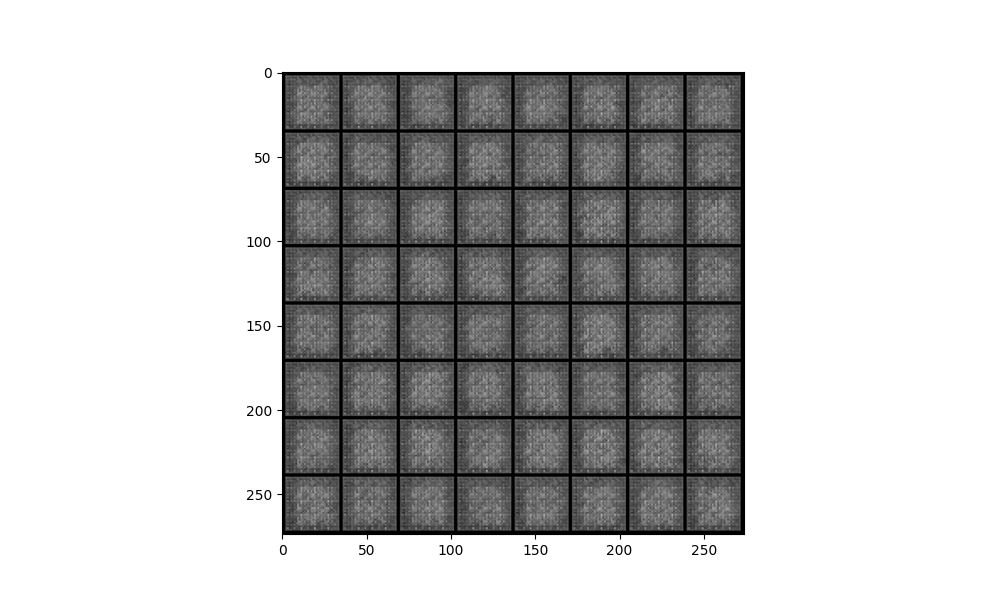
\includegraphics{./images/Pasted image 20231228114302.png}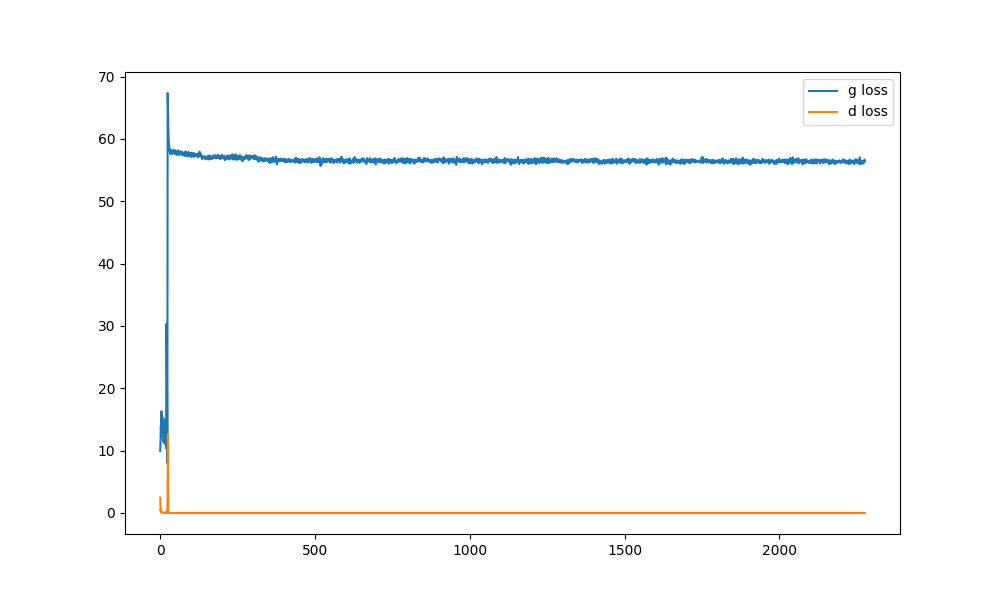
\includegraphics{./images/Pasted image 20231228114321.png}

\textbf{Change the learning rate of one or both models} Increasing the
learning rate of one or both the models will produce really bad results
and an unstable training: lr\_d=0.1
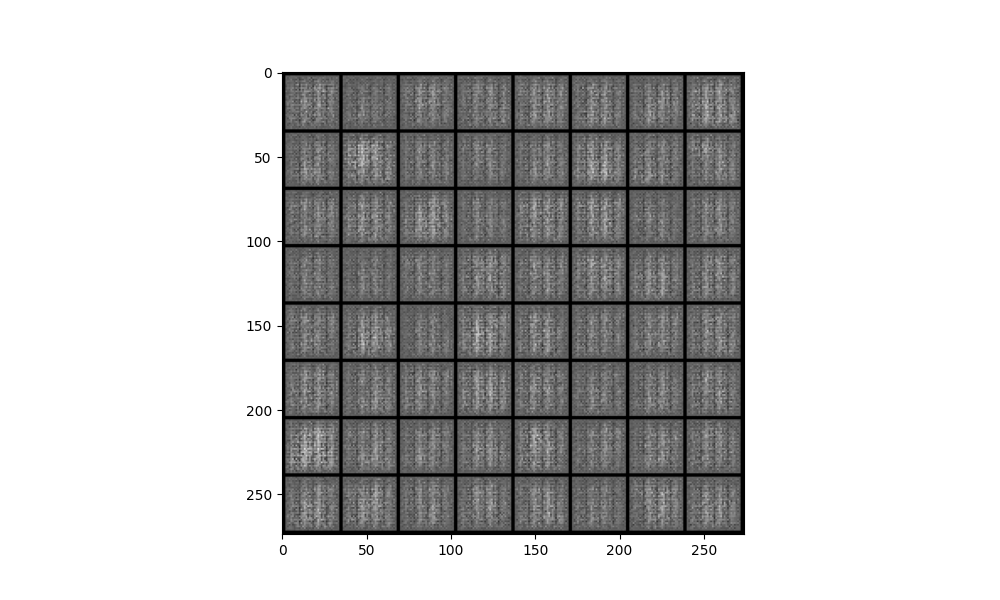
\includegraphics{./images/Pasted image 20231228114943.png}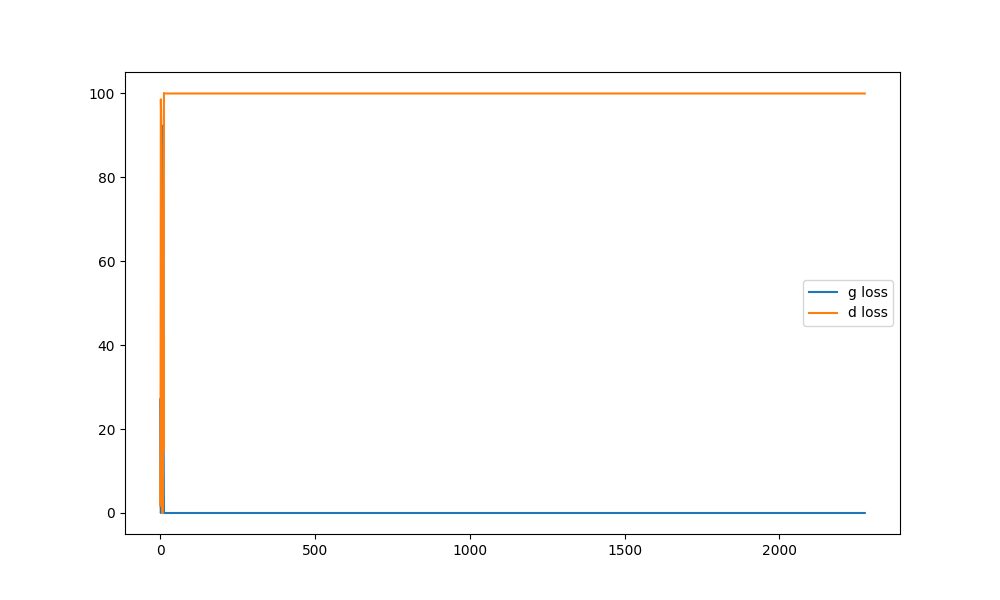
\includegraphics{./images/Pasted image 20231228115259.png}
lr\_d=0.1, lr\_g=0.1
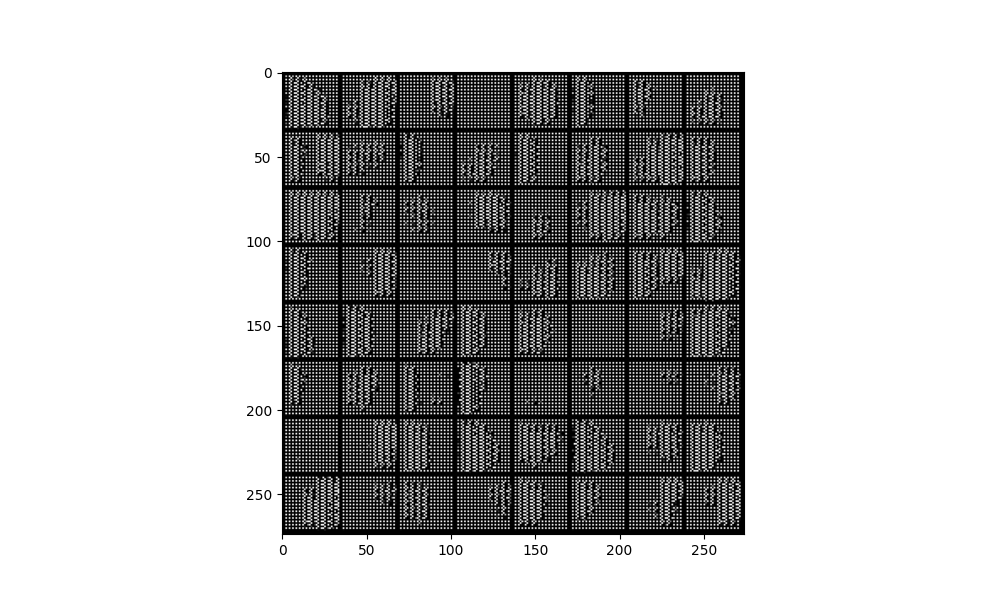
\includegraphics{./images/Pasted image 20231228115037.png}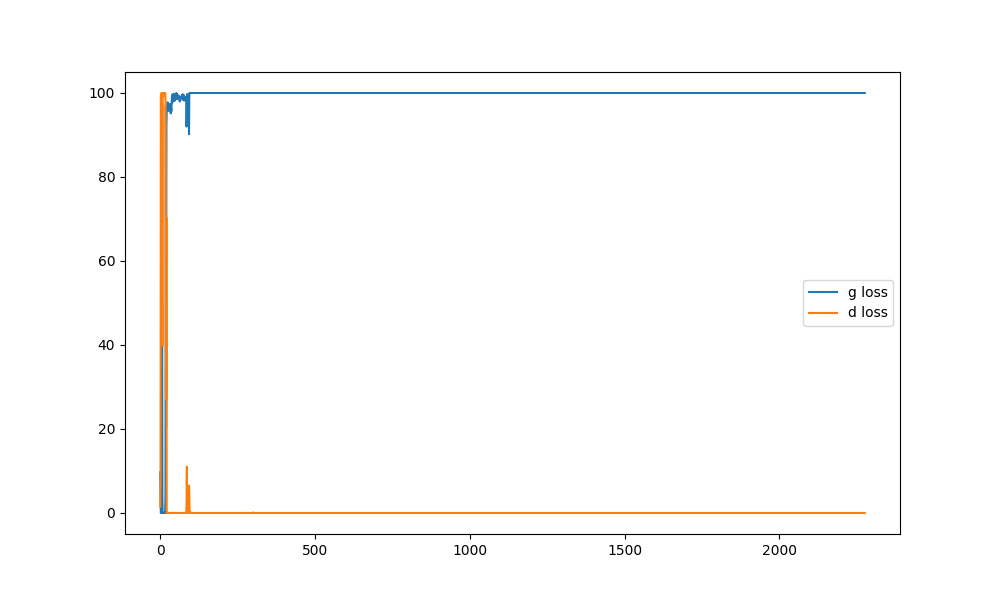
\includegraphics{./images/Pasted image 20231228115222.png}
lr\_g=0.1
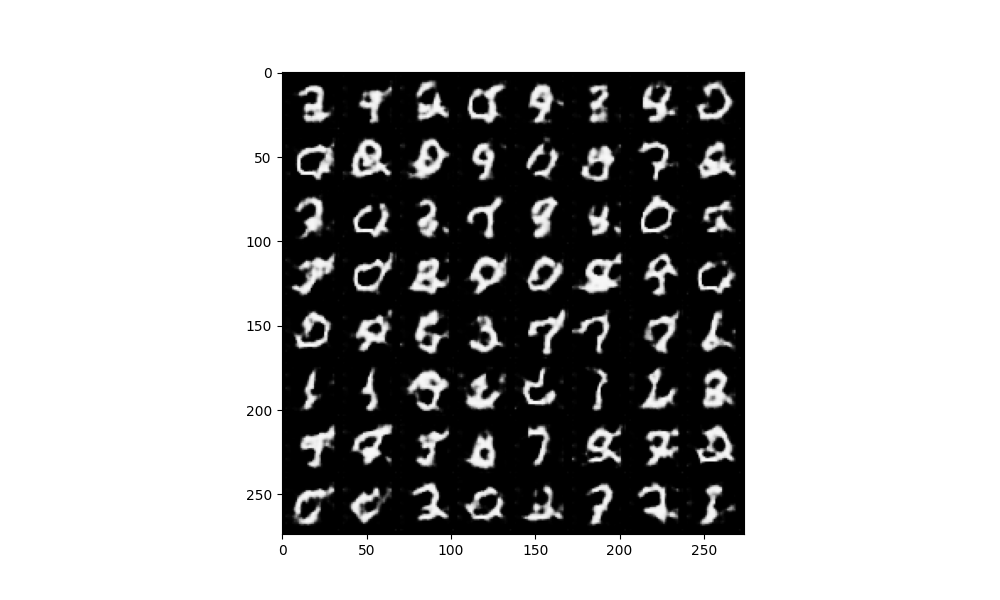
\includegraphics{./images/Pasted image 20231228115148.png}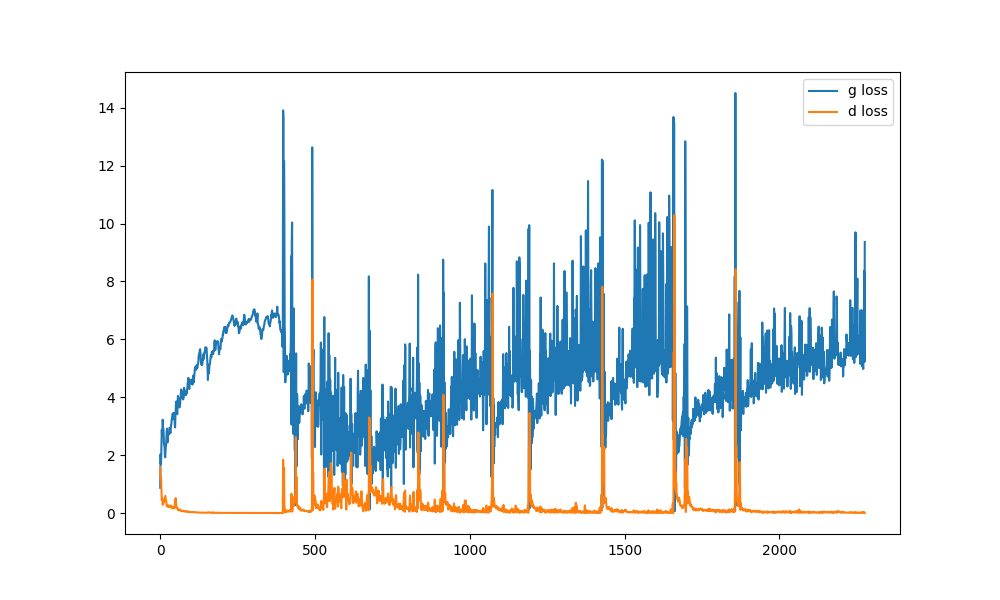
\includegraphics{./images/Pasted image 20231228115206.png}

Also decreasing the learning rate of both models will produce worse
results from baseline. In fact, we can see that the generator loss is
increasing while the discriminator loss is decreasing and this is the
opposite outcome that we would like to obtain. lr\_d=0.00002,
lr\_g=0.00005
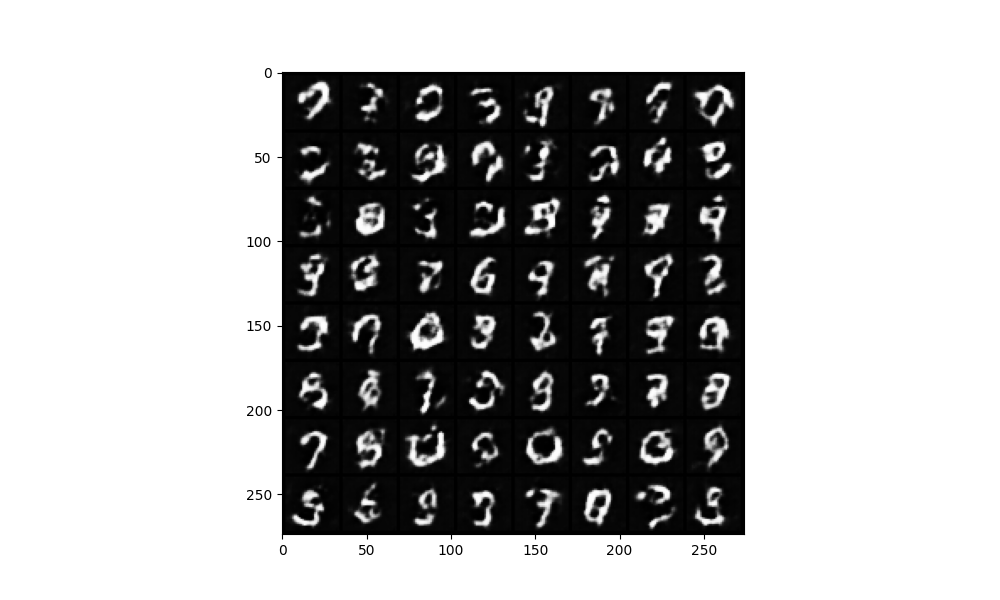
\includegraphics{./images/Pasted image 20231229113931.png}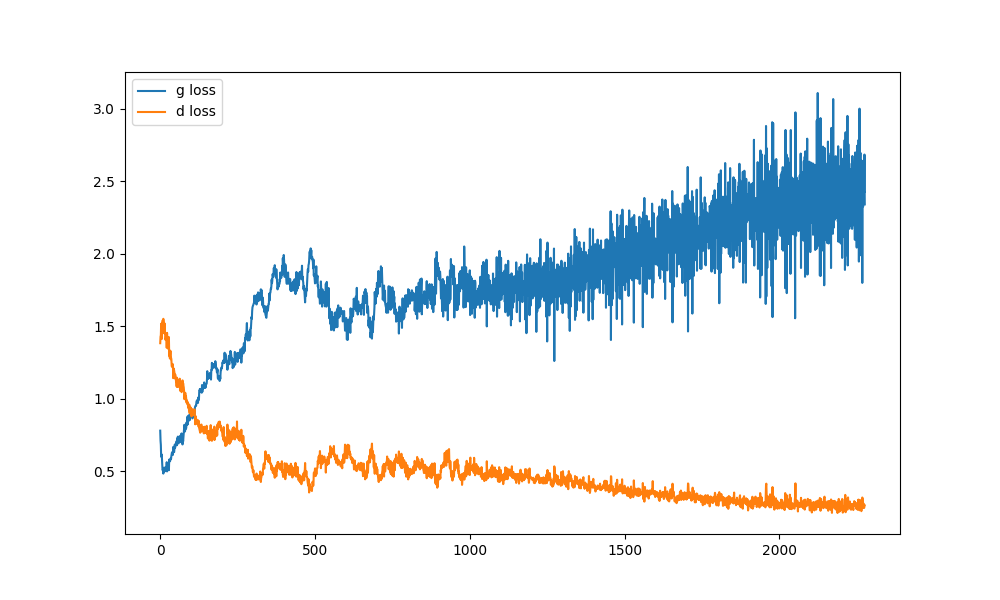
\includegraphics{./images/Pasted image 20231229114009.png}
lr\_d=0.000002, lr\_g=0.000005
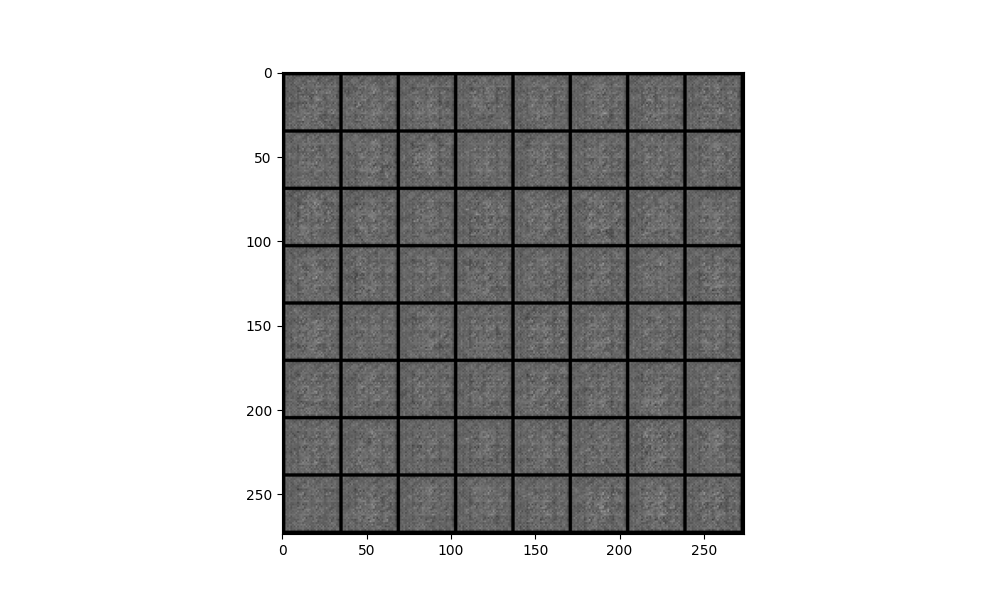
\includegraphics{./images/Pasted image 20231229114045.png}
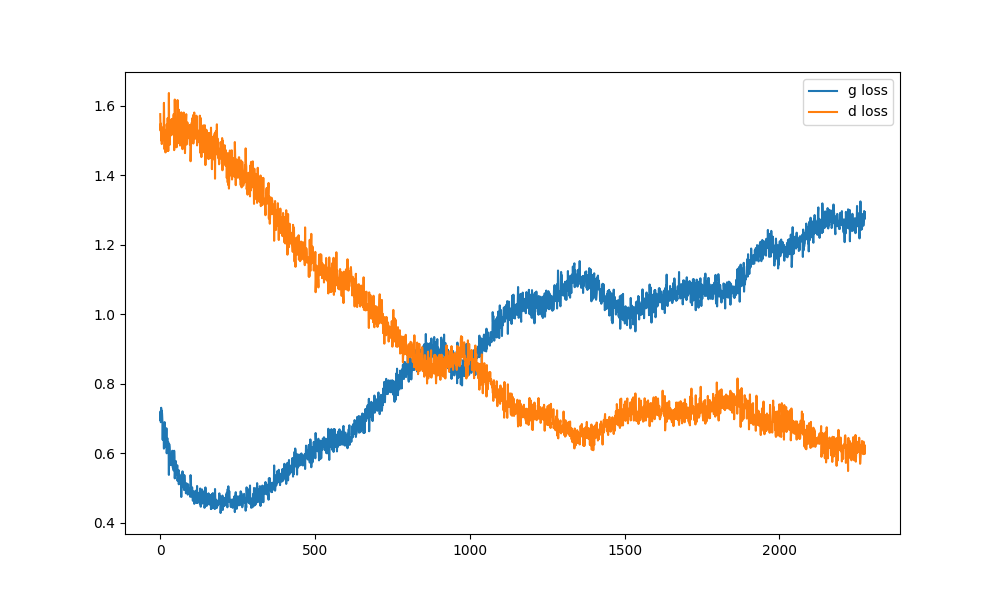
\includegraphics{./images/Pasted image 20231229114057.png}

\textbf{Learn for longer (ex : 30 epochs) even if it seems that the
model already generates correct images} After step 3000 we can see that
the training gets more unstable: the two losses experience periods of
diverging moment and then a spike. In our opinion, this could be the
effect of an exploding gradient phenomenon. Also the generator collapses
to producing a limited set of samples, ignoring the diversity present in
the training data. This is the ``mode collapse problem'' resulting in
generated samples that lack variety. We can see an extreme effect of
this problem in the test with epochs=100. epochs=30
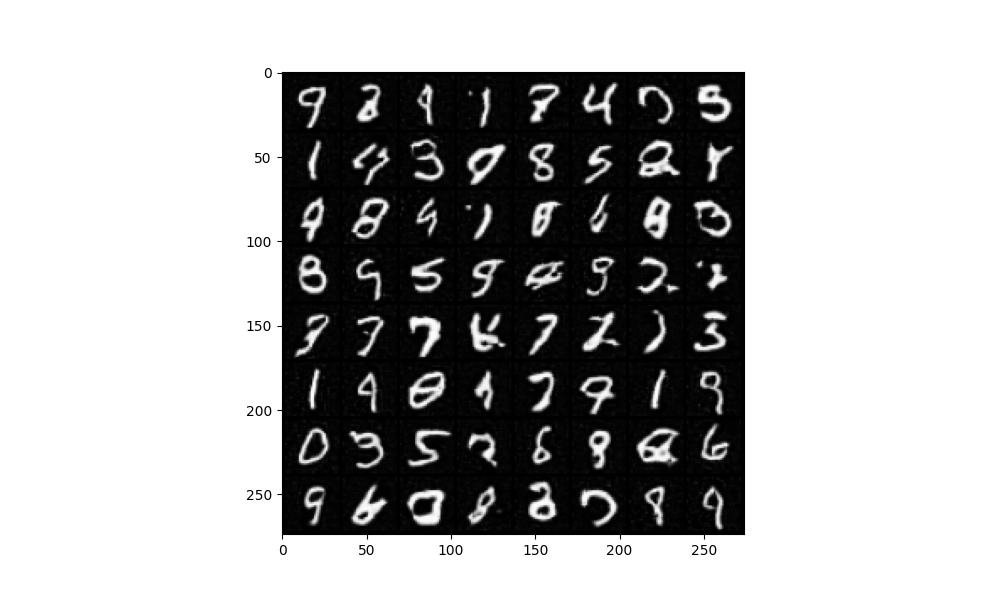
\includegraphics{./images/Pasted image 20231228115823.png}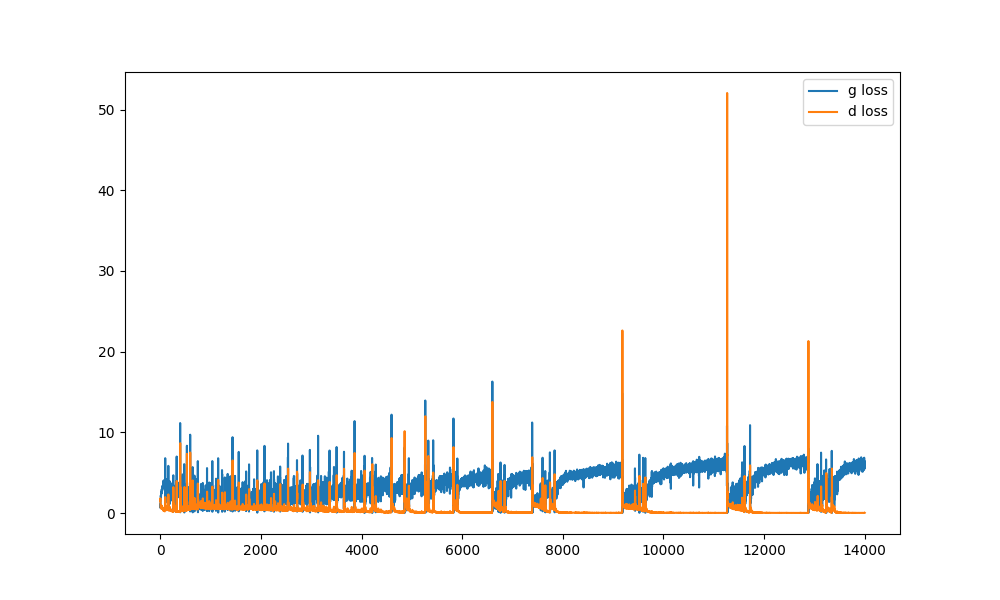
\includegraphics{./images/Pasted image 20231228115835.png}
epochs=100 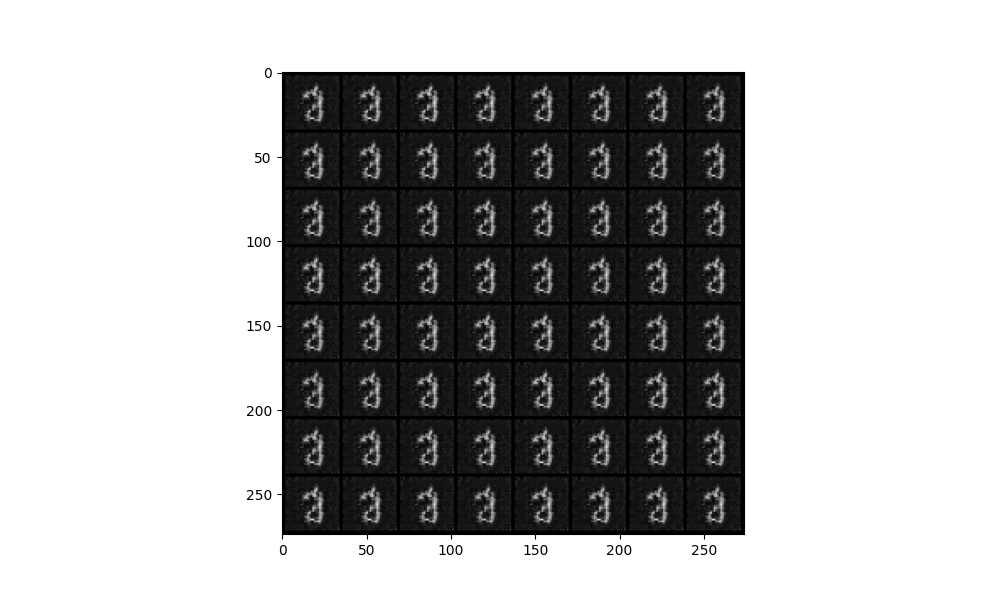
\includegraphics{./images/Pasted image 20231229114320.png}
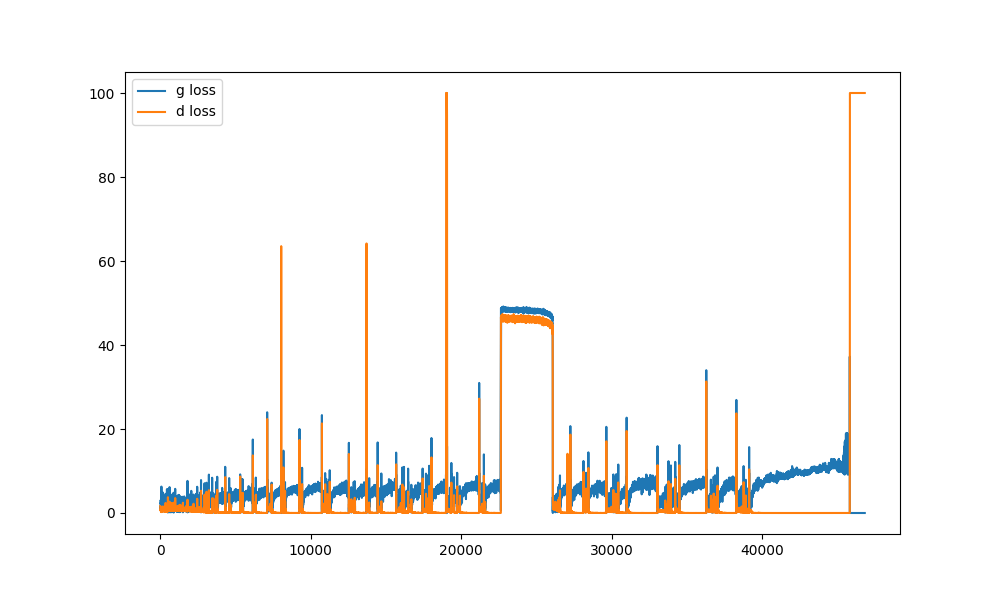
\includegraphics{./images/Pasted image 20231229114328.png}

\textbf{Reduce or increase significantly nz (ex : nz = 10 ou 1000)}
Increasing the nz significantly will make the training more unstable: a
very high-dimensional latent space might lead to overparameterization,
where the model has more parameters than necessary. Overparameterization
can make the training process slower and potentially lead to
overfitting. Also a larger latent space requires more diverse and
plentiful data to effectively capture the underlying data distribution.
If the dataset is not sufficiently large or diverse, the model might
struggle to learn meaningful representations. nz=100
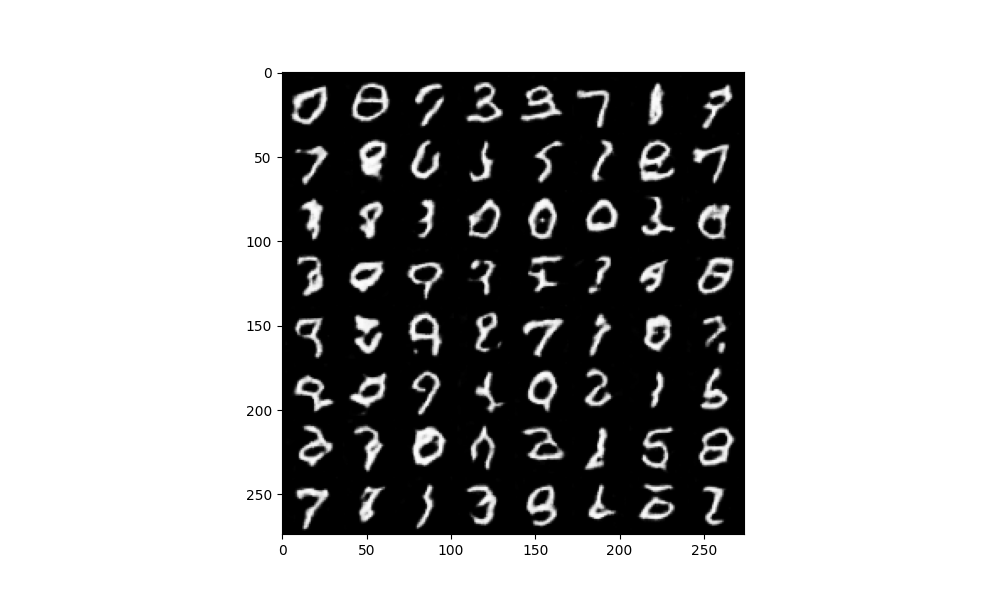
\includegraphics{./images/Pasted image 20231228120800.png}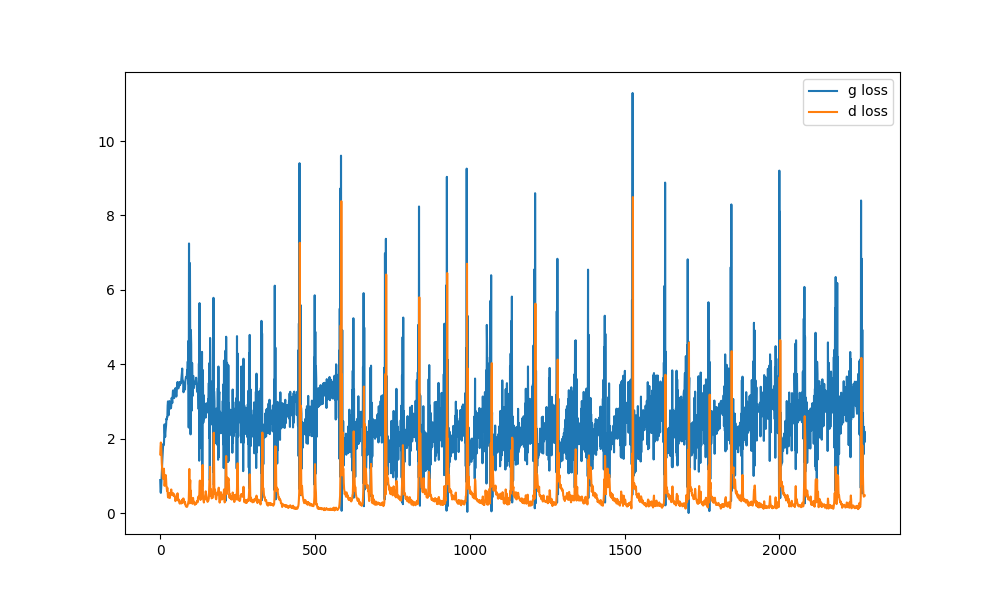
\includegraphics{./images/Pasted image 20231228121144.png}
If we decrease it, we obtain good results compared to the baseline. A
lower-dimensional latent space simplifies the model, making it
computationally more efficient and reducing the risk of overfitting.
With fewer parameters, the model might generalize better to unseen data.
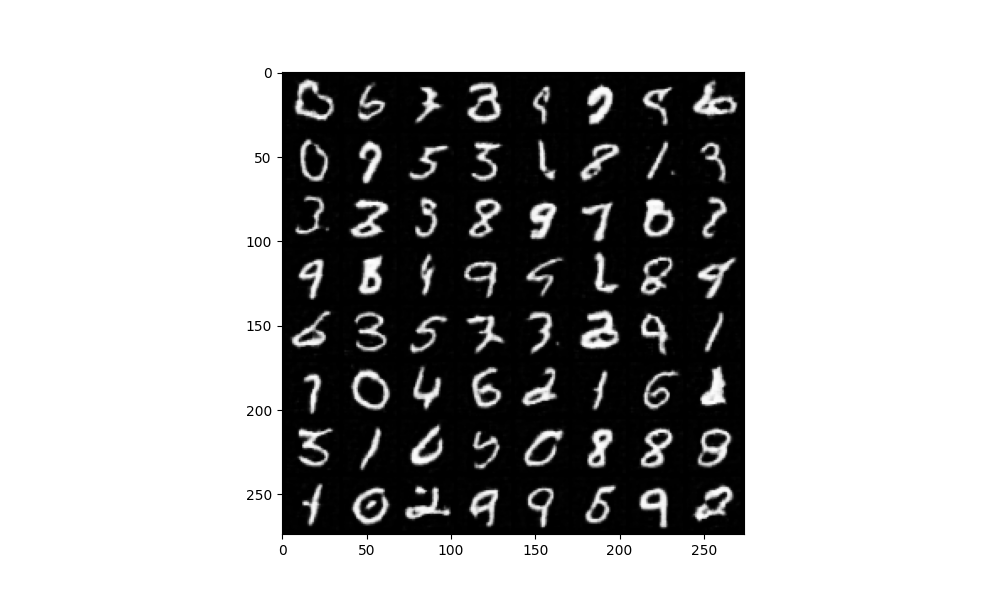
\includegraphics{./images/Pasted image 20231228121211.png}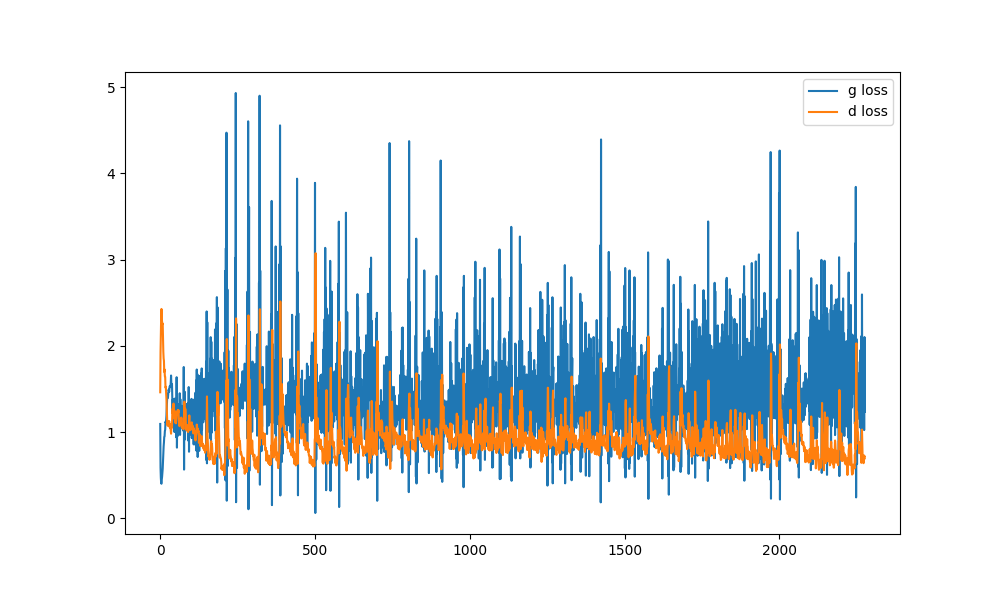
\includegraphics{./images/Pasted image 20231228121251.png}

\textbf{Replace the custom weight initialization with pytorch's default
initialization} Training with the default initialization will make us
obtain similar results as the baseline
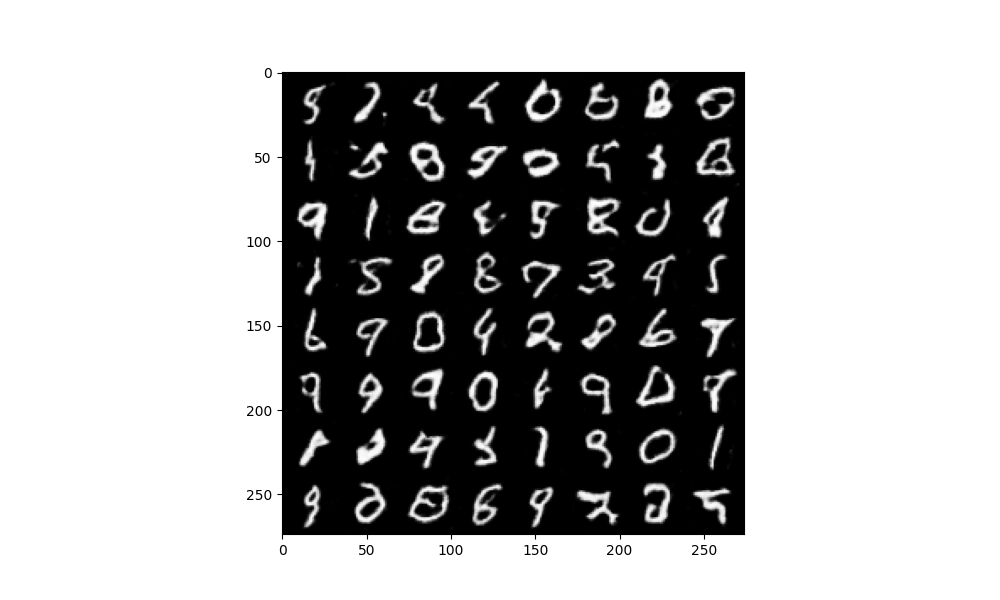
\includegraphics{./images/Pasted image 20231229115158.png}
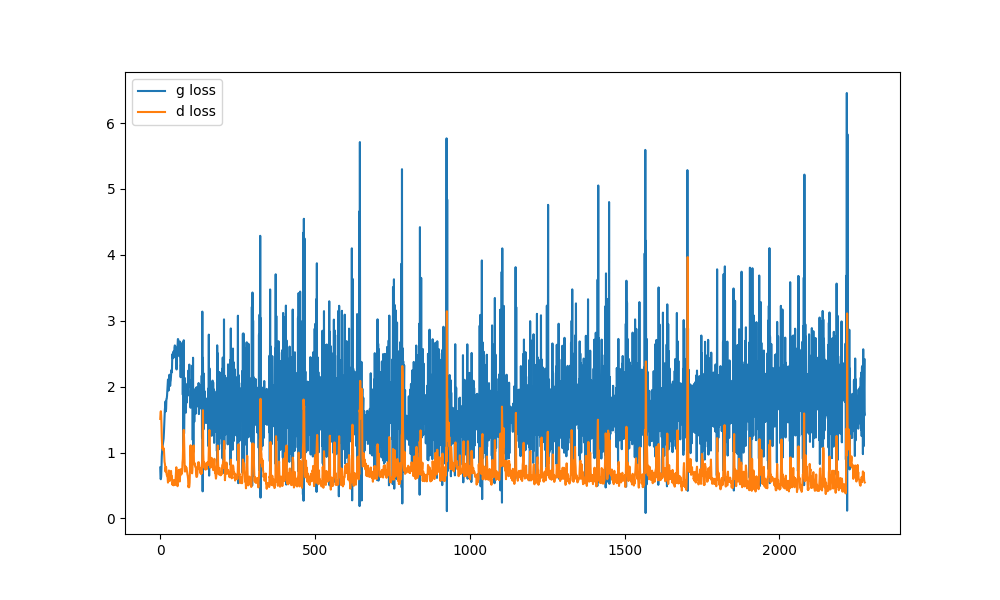
\includegraphics{./images/Pasted image 20231229115203.png}

\textbf{Using a learned GAN, take 2 noise vectors z1 and z2 and generate
the images corresponding to several linear interpolations
\(αz_1 + (1 − α)z_2, α ∈ [0, 1]\).} This technique serves to explore the
variety of results that a GAN can achieve. As \(\alpha\) varies from 0
to 1, the linear interpolation results in smooth transitions between the
generated images.
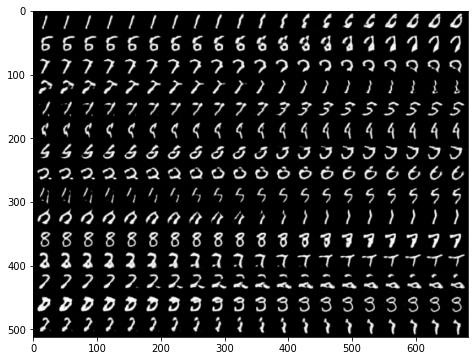
\includegraphics{./images/Pasted image 20231229115339.png}

\begin{center}\rule{0.5\linewidth}{0.5pt}\end{center}

\textbf{2 -- BONUS : Conditional Generative Adversarial Networks}

\hypertarget{comment-on-your-experiences-with-the-conditional-dcgan.}{%
\subsection{6. Comment on your experiences with the conditional
DCGAN.}\label{comment-on-your-experiences-with-the-conditional-dcgan.}}

We train a cDCGAN on MNIST using the image class as conditioning (with a
one-hot vector). The training of a conditioned GAN is more stable than
that of a traditional GAN. The images generated in the middle of the
training are more noisy; they exhibit numerous white points regardless
of the input vector, and this phenomenon is accompanied by higher
losses. At the end of our experiment, the generated images are of good
quality, and the networks seem to have stabilized.

\hypertarget{could-we-remove-the-vector-y-from-the-input-of-the-discriminator-so-having-cdx-instead-of-cdx-y}{%
\subsection{7. Could we remove the vector y from the input of the
discriminator (so having cD(x) instead of cD(x, y))
?}\label{could-we-remove-the-vector-y-from-the-input-of-the-discriminator-so-having-cdx-instead-of-cdx-y}}

It is important that the discriminator and generator have access to the
y label to generate a desired digit. If we remove the label y from the
discriminator inputs, the model will not learn to generate under a
condition. The generated numbers will be random like a normal GAN.
Additionally, experiments have demonstrated that this alteration
typically leads to a decrease in the model's performance. The inclusion
of y adds valuable contextual information that helps the discriminator
make more accurate decisions. Therefore, while simplifying the model by
removing y is an option, it's important to consider the potential
trade-offs in terms of effectiveness and accuracy.

\hypertarget{was-your-training-more-or-less-successful-than-the-unconditional-case-why}{%
\subsection{8. Was your training more or less successful than the
unconditional case ? Why
?}\label{was-your-training-more-or-less-successful-than-the-unconditional-case-why}}

Our training was more successful in the conditional case compared to the
unconditional one, since the conditional variable helps refining the
learning process. The training seems to be smoother and more effective,
with less high spikes compared to the baseline of the unconditional gan.
Also, in the end the discriminator loss is going upwards, while the
generator loss is still decreasing and this is the behavior that we want
to achieve.

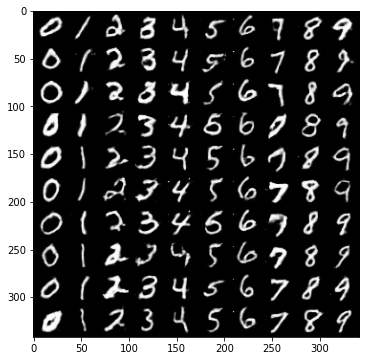
\includegraphics{./images/Pasted image 20231229115925.png}
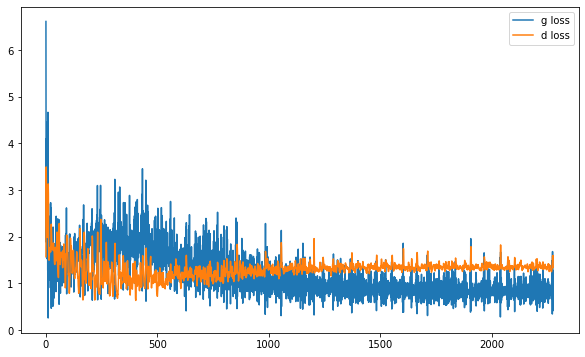
\includegraphics{./images/Pasted image 20231229115930.png}

\hypertarget{test-the-code-at-the-end.-each-column-corresponds-to-a-unique-noise-vector-z.-what-could-z-be-interpreted-as-here}{%
\subsection{9. Test the code at the end. Each column corresponds to a
unique noise vector z. What could z be interpreted as here
?}\label{test-the-code-at-the-end.-each-column-corresponds-to-a-unique-noise-vector-z.-what-could-z-be-interpreted-as-here}}

As seen from the generation, the latent vector z only changes the style
of the generated image. Since we have given the condition and it learns
according to that, the output image is from the same category/class.
This can be seen from the image.
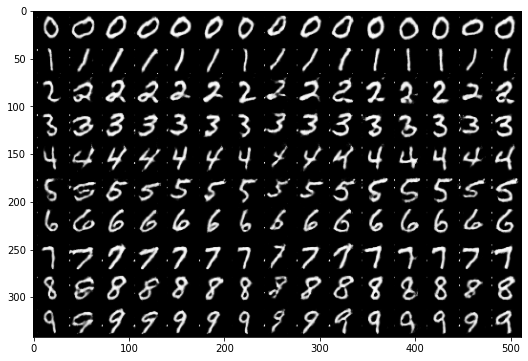
\includegraphics{./images/Pasted image 20231229115737.png}
